\chapter{Background}
The goal of this project is to build a benchmark framework for stream processing systems, which aim to solve issues related to \textbf{V}elocity and \textbf{V}ariety of big data\cite{GameChanger}. In order to process continuously incoming data with a low latency, both the data and stream processing task have to be distributed. Usually the data is stored in a distributed storage system which consists of a set of data nodes. A distributed storage system could be a distributed file system, for example HDFS(\cref{subsection:hdfs}), or distributed messaging system such as Kafka discussed in \cref{subsection:kafka}. The stream processing task is divided into a set of sub-tasks which are distributed in a computer cluster(see \cref{subsection:computing_cluster}). The nodes in a computer cluster read data from distributed storage system and execute sub-tasks in parallel. Which achieves both data parallelism and task parallelism of parallel computing which is discussed in \cref{subsection:parallel_computing}.
 
In \cref{section:benchmark}, we present several widely accepted benchmarks of DBMS, cloud services and graph processing systems. There are many good features of the design and implementation of these benchmarks and some of them could be used in our benchmark as well. At the end, we discuss an existing benchmark of stream processing systems -- \texttt{The Yahoo Streaming Benchmark}. 
 

\section{Cloud Computing}
Cloud computing, also known as ``on-demand computing'', is a kind of Internet-based computing, where shared resources, data and information are provided to computers and other devices on-demand. It is a model for enabling ubiquitous, on-demand access to a shared pool of configurable computing resource\cite{neto2011demystifying, mell2011nist}. Cloud computing and storage solutions provide users and enterprises with various capabilities to store and process their data in third-party data centers\cite{haghighat2015cloudid}. Users could use computing and storage resources as need elastically and pay according to the amount of resources used. In another way, we could say cloud computing technologies is a collection of technologies to provide elastic ``pay as you go'' computing. That includes scalable file system and data storage such as Amazon S3 and Dynamo, scalable processing such as MapReduce and Spark, visualization of computing resources and distributed consensus. 

% Maybe we could have pictures here to show the difference between
% serial computing and parallel computing
\subsection{Parallel Computing}
\label{subsection:parallel_computing}
Parallel computing is a computational way in which many calculations participate and simultaneously solve a computational problem, operating on the principle that large problems could be divided into smaller ones and smaller problems could be solved at the same time. As mentioned in the beginning of this chapter, both data parallelism and task parallelism are achieved during stream processing. Besides, base on the level of parallelism there are two other types of parallel computing: bit-level parallelism and instruction-level parallelism. In the case of bit-level and instruction-level parallelism, parallelism is transparent to the programmer. Compared to serial computation, parallel computing has the following features: multiple CPUs, distributed parts of the problem, concurrent execution on each compute node. Because of these features, parallel computing could obtain better performance than serial computing. 

% discuss scaling up and scaling out 
Parallel computers can be roughly classified according to the level at which the hardware supports parallelism, with multi-core and multi-processor computers having multiple processing elements within a single machine, while clusters, MPPs, and grids use multiple computers to work on the same task. Therefore, when the need for parallelism arises, there are two different ways to do that. The first way is ``Scaling Up", in which a single powerful computer is added with more CPU cores, more memory, and more hard disks. The other way is dividing task between a large number of less powerful machines with (relatively) slow CPUs, moderate memory amounts, moderate hard disk counts, which is called "Scaling out". Compare to ``Scaling up'', ``Scaling out'' is more economically viable. Scalable cloud computing is trying to exploiting ``Scaling Out" instead of ``Scaling Up".

% figure to show computer cluster
\subsection{Computer Cluster}
\label{subsection:computing_cluster}
The ``Scaling Out" strategy turns out computer cluster. A computer cluster consists of a set of computers which are connected to each other and work together so that, in many respects, they can be viewed as a single system. The components of a cluster are usually connected to each other through fast local area networks ("LAN"), with each node running its own instance of an operating system. In most circumstances, all of the nodes use the same hardware and the same operating system and are set to perform the same task, controlled and scheduled by software. The large number of less powerful machines mentioned above is a computer cluster.

% task scheduling
% node failure
One common kind of clusters is master-slave cluster which has two different types of nodes, master nodes and slave nodes. Generally,  users only interact with the master node which is a specific computer managing slaves and scheduling tasks. Slave nodes are not available to users which makes the whole cluster as a single system.
% It is possible that each nodes in a cluster could be failed with some probability. To avoid master node be the single point of failure, master server may be further divided to active master and standby master (passive master) in order to meet the requirement of fault tolerance. When a slave node failed, master node will reassign the running task in the failed node to another slave node. 

As the features of computing cluster demonstrated above, it is usually used to improve performance and availability over that of a single computer. In most cases, the average computing ability of a node is less than a single computer as scheduling and communication between nodes consume resources.

% table compare batch and stream processing
% table to show S4, MapReduce, Spark, Storm
\subsection{Batch Processing and Stream Processing}
According to the size of data processed per unit, processing model could be classified to two categories: batch processing and stream processing. Batch processing is very efficient in processing high \textbf{V}olume data. Where data is collected as a dataset, entered to the system, processed as a unit.  The output is another data set that can be reused for computation. Depending on the size of the data being processed and the computational power of the computer cluster, the latency of a task could be measured in minutes or more. Since the processing unit of batch processing is a dataset, any modification such as incorporating new data of an existing dataset turns out a new dataset and the whole computation need start again. MapReduce and Spark are two widely used batch processing models.
 
In contrast, stream processing emphasizes on the \textbf{V}elocity of big data. It involves continual input and outcome of data. Each records in the data stream is processed as a unit. Therefore, data could be processed within small time period or near real time. Streaming processing gives decision makers the ability to adjust to contingencies based on events and trends developing in real-time. Beside low-latency, another key feature of stream processing is incremental computation, whenever a piece of new data arrives, attempts to save time by only recomputing those outputs which ``depend on" the incorporating data without recomputing from scratch.

% Mini-batch
Except batch processing and stream processing, between them there is another processing model called mini-batch processing. Instead of processing the streaming data one record at a time, mini-batch processing model discretizes the streaming data into tiny, sub-second mini-batches. Each mini-batch is processed as a batch task. As each batch is very small, mini-batch processing obtains much better latency performance than batch processing.

\begin{table}[H] %\centering
\begin{tabular}{p{3.2cm} p{4.2cm} p{4.2cm}} 
% Alignment of sells: l=left, c=center, r=right. 
% If you want wrapping lines, use p{width} exact cell widths.
% If you want vertical lines between columns, write | above between the letters
% Horizontal lines are generated with the \hline command:
\toprule % The line on top of the table
  & Batch  & Stream \\ 
\hline 
% Place a & between the columns
% In the end of the line, use two backslashes \\ to break the line
% contents of the cell
 {\small Latency} & {\small mins - hours} & {\small milliseconds - seconds} \\
 {\small Throughput} & {\small Large} & {\small Small(relatively)}\\
 {\small Prior \textbf{V}} & {\small Volume} & {\small Velocity}\\   
\bottomrule
\end{tabular} % for really simple tables, you can just use tabular
% You can place the caption either below (like here) or above the table
\caption{Comparison of batch processing and stream process} 
% Place the label just after the caption to make the link work
\label{table:BatchVSStream}
\end{table}

\subsection{MapReduce}
MapReduce is a parallel programming model and an associated implementation for processing and generating large data sets with a parallel, distributed algorithm on a cluster  of commodity hardware in a reliable, fault-tolerant manner\cite{dean2008mapreduce}. To achieve the goal, there are two primitive parallel methods (map and reduce) predefined in MapReduce programming model. A MapReduce job usually executes map tasks first to split the input data-set into independent chunks and perform map operations on each chuck in a completely parallel manner. In this step,  MapReduce can take advantage of locality of data, processing it on or near the storage assets in order to reduce the distance over which it must be transmitted. The final outputs of map stage are shuffled as input of reduce tasks which performs a summary operation. 

Usually, the outputs of map stage are a set of key/value pairs. Then the outputs are shuffled to reduce stage base on the key of each pair. The whole process of MapReduce could be summarized as following 3 steps:
\begin{itemize}
  \item \textbf{Map:} Each worker node reads data from cluster with lowest transmit cost and applies the "map()" function to the local data, and writes the output to a temporary storage. 
  \item \textbf{Shuffle:} Worker nodes redistribute data based on the output keys (produced by the "map()" function), such that all data belonging to one key is located on the same worker node.
  \item \textbf{Reduce:}Worker nodes now process each group of output data, per key, in parallel.
\end{itemize}

One good and widely used MapReduce implementation is the Hadoop~\footnote{\url{http://hadoop.apache.org/}} MapReduce \cite{MapReduce} which consists of a single master JobTracker and one slave TaskTracker per cluster-node. The programming models of many stream processing systems like Storm, Flink and Spark Streaming are all inspired from MapReduce. Operators \texttt{Map} and \texttt{Reduce} are either built-in these systems or could be implemented with provided built-in APIs. For example, Flink supports \texttt{Map}, \texttt{Reduce} and some other MapReduce-inspired operations like \texttt{FlatMap}, \texttt{Filter} by default. In Storm, all these mentioned operators could be implemented with APIs of \texttt{Spout} and \texttt{Bolt}.

%The master is responsible for scheduling the jobs' component tasks on the slaves, monitoring them and re-executing the failed tasks to achieve fault tolerance. More specifically, fault tolerance in MapReduce is provided from two aspects: task failure that can be monitored by passing heartbeat message periodically between JobTracker and TaskTracker, JobTracker failure that can be guaranteed by the approach of checking point. Checking point is an approach for applications to recover from failure by taking the snapshot of current intermediate results, resource allocation and related information to file system. When a JobTracker starts up, it looks for such data, so that it can restart work from where it left off.


\subsection{Hadoop Distribution File Systems}
\label{subsection:hdfs}

%\begin{figure}
%  \begin{center}
%  \subfigure{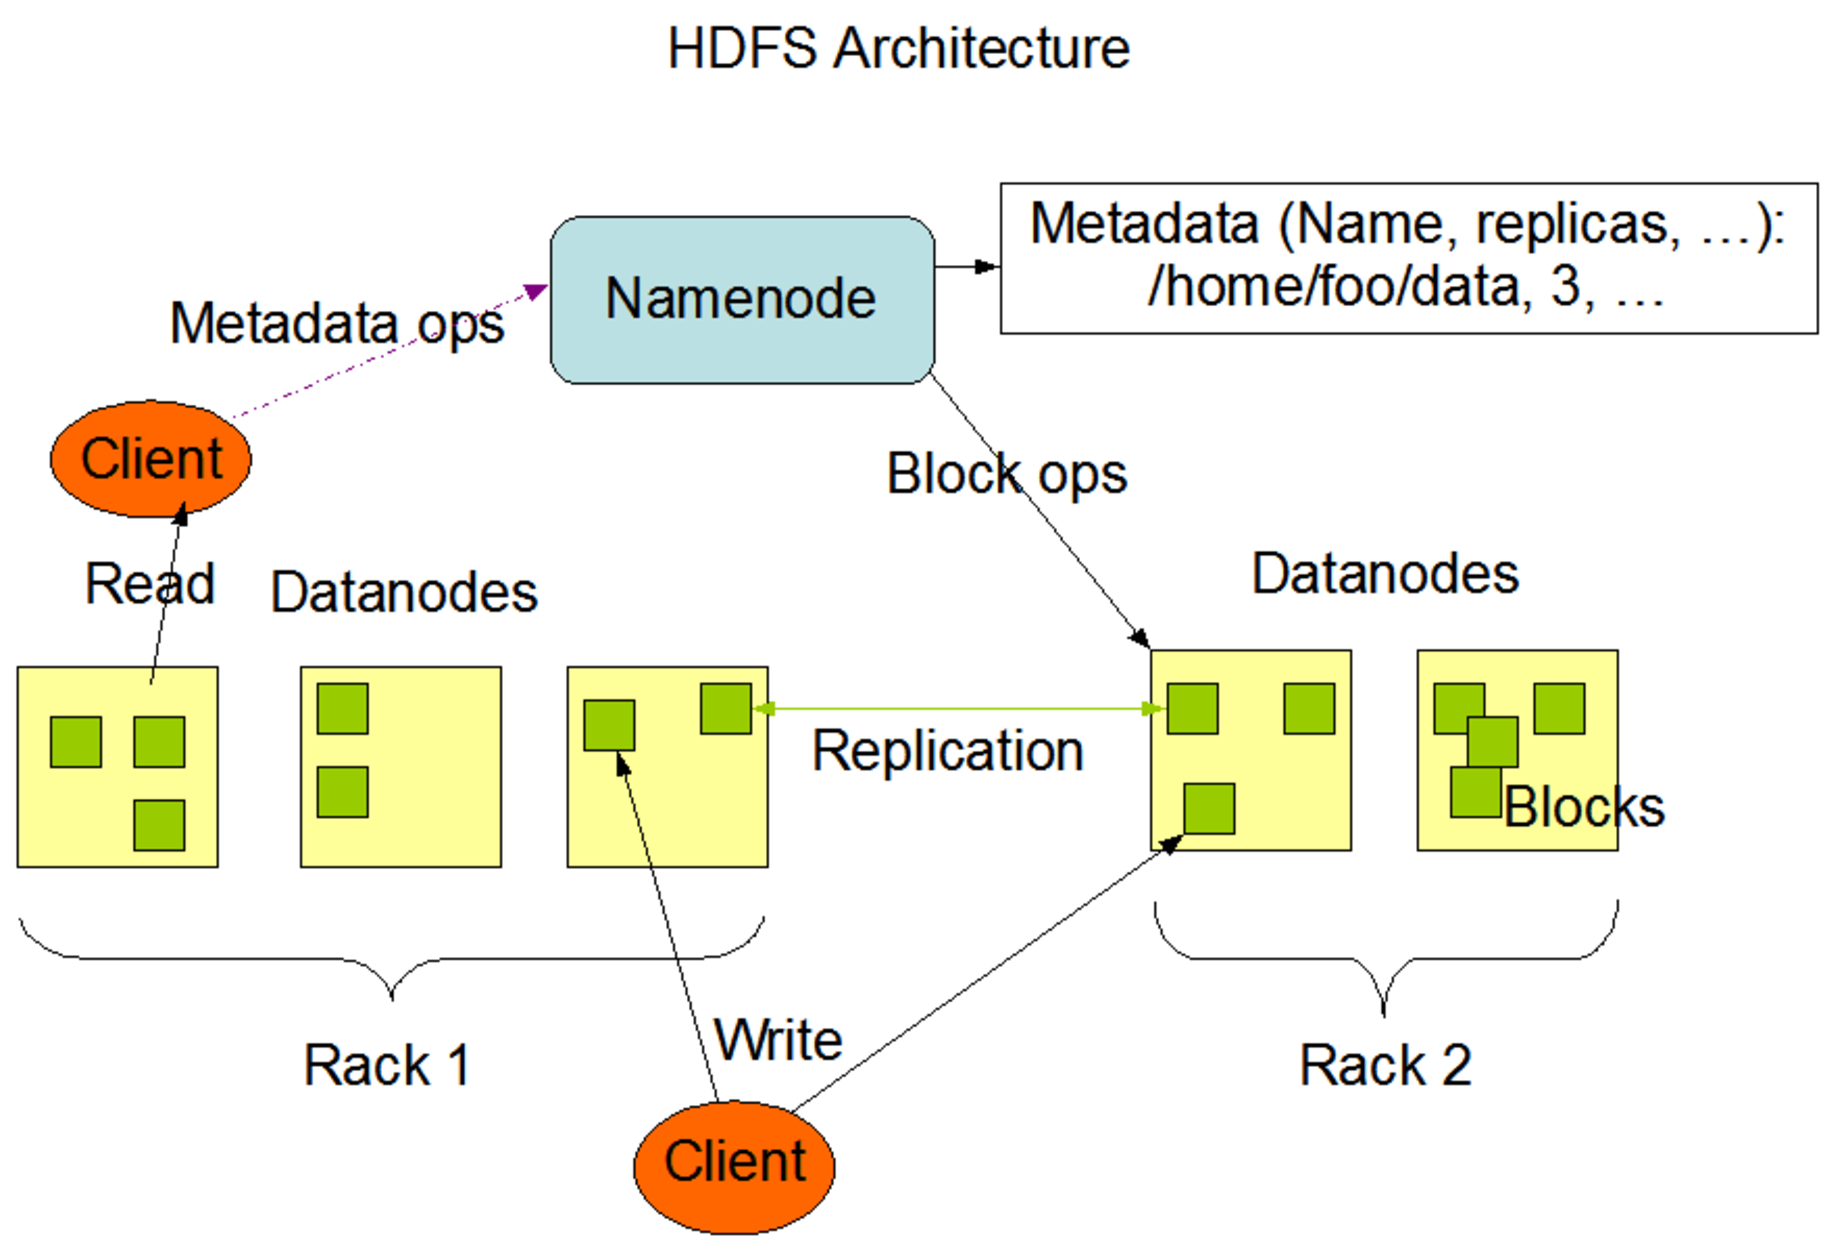
\includegraphics[scale=0.35]{images/hdfsarchitecture}}
%   \caption{HDFS architecture \cite{HDFS}}
%   \label{fig:hdfs_architecture}
%  \end{center}
%\end{figure}

Hadoop Distributed File System \cite{HDFS} is open source clone of Google File System (GFS) \cite{ghemawat2003google} that is deployed on computing cluster. In Hadoop MapReduce framework, locality relies on Hadoop Distributed File System (HDFS) that can fairly divide input file into several splits across each worker in balance. In another word, MapReduce is built on the distributed file system and executes read/write operations through distributed file system. HDFS is highly fault-tolerant and is designed to be deployed on low-cost hardware. HDFS provides high throughput access to application data and is suitable for applications that have large data sets. HDFS relaxes a few POSIX requirements to enable streaming access to file system data. \cite{HDFS} The assumptions and goals of HDFS includes: hardware failure, high throughput, large dataset, streaming access, data load balance and simple coherency model, "Moving Computation is Cheaper than Moving Data", and portability across heterogeneous hardware and software platforms. 

%An HDFS instance may consist of hundreds or thousands of nodes, each handling part of the file system's data. Therefore, HDFS could store very large dataset and provide high throughput. 
%Normally, the failure probability of a machine is non-trivial. But in a cluster with thousands machines, some nodes would be always non-functional. From Figure~\ref{fig:hdfs_architecture} it is clear to know that HDFS architecture is master-slaves architecture with a namenode and multi datanodes. Based on this architecture, any crashed datanode can be checked out by sending heartbeat messages periodically to namenode. Once certain datanode fail to send heartbeat message to namenode within regulated time period, namenode would mark that datanode inactive and ask other datanodes to replicate data on the failed datanode. When free space on certain servers are below the threshold specified on the configuration file, other datanodes are also asked to replicate data on overhead datanode to achieve data load balance. HDFS applications need a write-once-read-many access model for files. A file once created, written, and closed need not be changed. This assumption simplifies data coherency issues and enables high throughput data access.\cite{HDFS} A computation is much more efficient if it is executed in the same node or near the node where the request data located. Because transmission of data takes much more time than changing a server to do a computation. Base on this assumption, HDFS provides interfaces for applications to move themselves closer to where the data is located. In addition, one more thing in the respect of fault tolerance is referred. The principle of fault tolerance in HDFS refers to checkpoint and then HDFS recovers data from checkpoint at certain time point when certain slave server is crashed down.

In general, HDFS and MapReduce always works together. In a distribute cluster, each datanode in HDFS runs  a TaskTracker as a slave node in MapReduce. MapReduce retrieves data from HDFS and executes computation and finally writes results back to HDFS.

\subsection{Kafka}
\label{subsection:kafka}

\begin{figure}
  \begin{center}
  \subfigure{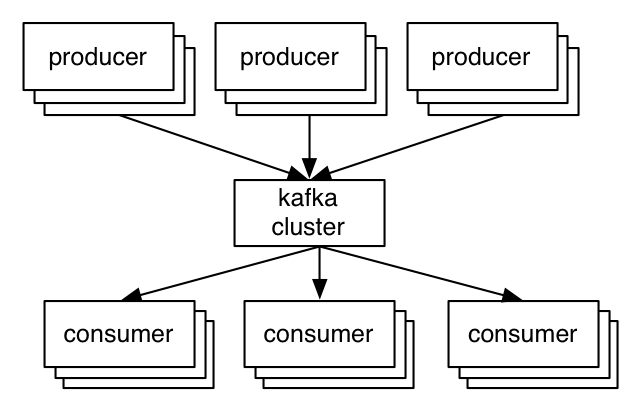
\includegraphics[scale=0.75]{images/kafka_producer_consumer}}
   \caption{Kafka producer and consumer \cite{Kafka}}
   \label{fig:kafka_producer_consumer}
  \end{center}
\end{figure}

Apache Kafka is a high-throughput distributed publish-subscrib messing system which was originally developed by LinkedIn. Now it is one top level project of the Apache Software Foundation. It aims to provide a unified, high-throughput, low-latency platform for handling continuous data feeds. A stream processing system subscribes from Kafka will get notified within very short time after a publisher publishes something. In StreamBench, we use Kafka provide messaging service. Before we go into architecture of Kafak, there are some basic messaging terminologies: \cite{Kafka}

\begin{itemize}
  \item \textbf{Topic:} Kafka maintains feeds of messages in categories called topics. 
  \item \textbf{Producer:} Processes that publish messages to a Kafka topic are called producers.
  \item \textbf{Consumer:} Processes that subscribe to topics and process the feed of published messages are consumers.
   \item \textbf{Broker:} Kafka is run as a cluster comprised of one or more servers each of which is called a broker.
\end{itemize}

As Figure~\ref{fig:kafka_producer_consumer} shown, producers send messages over the network to the Kafka cluster which holds on to these records and hands them out to consumers. More specifically, producers publish their messages to a topic, and consumers subscribe to one or more topics. Each topic could have multiple partitions that are distributed over the servers in Kafka cluster, allowing a topic to hold more data than storage capacity of any server. Each partition is replicated across a configurable number of servers for fault tolerance. Each partition is an ordered, immutable sequence of messages that is continually appended to a log. The messages in the partitions are each assigned a sequential id number called the offset that uniquely identifies each message within the partition.  Figure ~\ref{fig:kafka_partitioned_topic} shows a producer process appending to the logs for the two partitions, and a consumer reading from partitions sequentially. 

At a high-level Kafka gives the following guarantees: \cite{Kafka}
\begin{itemize}
  \item Messages sent by a producer to a particular topic partition will be appended in the order they are sent. That is, if a message M1 is sent by the same producer as a message M2, and M1 is sent first, then M1 will have a lower offset than M2 and appear earlier in the log. 
  \item A consumer instance sees messages in the order they are stored in the log.
  \item For a topic with replication factor N, we will tolerate up to N-1 server failures without losing any messages committed to the log.
\end{itemize}


Another very important feature of Kafka is messages with the same key will be sent to the same partition. When a distributed application consumes data from a kafka topic in parallel,  data with the same key goes to the same executor which could avoid data shuffle.
% kafka guarantees that data with same key will be sent to the same partition


\begin{figure}
  \begin{center}
  \subfigure{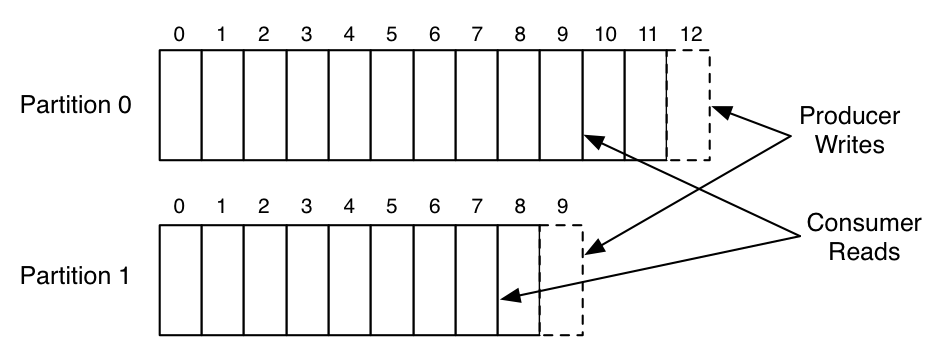
\includegraphics[scale=0.75]{images/partitioned_log}}
   \caption{Kafka topic partitions}
   \label{fig:kafka_partitioned_topic}
  \end{center}
\end{figure}
% \subsection{Zookeeper}
% ZooKeeper is a centralized service for maintaining configuration information, naming, providing distributed synchronization, and providing group services. All of these kinds of services are used in some form or another by distributed applications. Each time they are implemented there is a lot of work that goes into fixing the bugs and race conditions that are inevitable. Because of the difficulty of implementing these kinds of services, applications initially usually skimp on them ,which make them brittle in the presence of change and difficult to manage. Even when done correctly, different implementations of these services lead to management complexity when the applications are deployed.

\section{Benchmark}
\label{section:benchmark}

As system advanced and complicated, it became more difficult to compare the performance of various systems simply by looking at their specifications. For one kind of systems, there are always a sequence of performance metrics which indicate the performance of a specific system, such as average response time of a query in DBMS. In computing, a benchmark is the act of running a set of programs mimicking a particular type of workload on a system, in order to assess the relative performance metrics of a system. Many benchmarks are designed and widely used in industry to compare systems.

In this Section, we discuss benchmarks for different computer systems: DBMS, Cloud Data Service and Graph Processing System. An existing benchmark of Stream processing system developed by Yahoo is also present in \cref{subsection:ysb}. 

\subsection{Traditional Database Benchmarks}
Traditional database management systems were evaluated with industry standard benchmarks like TPC-C\cite{TPC-C}, TPC-H\cite{TPC-H}. These have focused on simulating complete business computing environment where plenty of users execute business oriented ad-hoc queries that involve transactions, big table scan, join, and aggregation. The queries and the data populating the database have been chosen to have broad industry-wide relevance. This benchmark illustrates decision support systems that examine large volumes of data, execute queries with a high degree of complexity, and give answers to critical business questions\cite{TPC-H}. The integrity of the data is verified during the process of the execution of the benchmark to check whether the DBMS corrupt the data. If the data is corrupted, the benchmark measurement is rejected entirely\cite{dey2014ycsb+t}. Benchmark systems for DBMS mature, with data and workloads simulating real common business use cases, they could evaluate performance of DBMS very well. Some other works were done related to specific business model. 

Linkbench \cite{LinkBench} benchmarks database systems which store ``social network" data specifically. The workloads of database operations are based on Facebook's production workload and the data is also generated in such a way that key properties of the data match the production social graph data in Facebook. LinkBench provides a realistic and challenging test for persistent storage of social and web service data. 

\subsection{Cloud Service Benchmarks}
As the data size keep increasing, traditional database management systems could not handle some use cases with very big size data very well. To solve this issue, there are plenty of NoSQL database systems developed for cloud data serving. With the widespread use of such cloud services, several benchmarks are introduced to evaluate these cloud systems.

One widely used and accepted extensible cloud serving benchmark named \textit{Yahoo! Cloud Servicing Benchmark}(YCSB) developed by Yahoo\cite{YCSB}. It  proposes two benchmark tiers for evaluating the performance and scalability of cloud data serving systems such as Cassandra, HBase, and CouchDB. A core set of workloads are developed to evaluate different tradeoffs of cloud serving systems. Such as write/read heavy workloads to determine whether system is write optimised or read optimised. To evaluate transaction features in later NoSQL database,  YCSB+T \cite{dey2014ycsb+t} extends YCSB with a specific workload for transaction called Closed Economy Workload(CEW). A validation phase is added to the workload executor to check consistency of these cloud databases. YCSB++ \cite{ycsb++} is another set of extensions of YCSB to benchmark other five advance features of cloud databases such as bulk insertions, server-side filtering. YCSB++ could run multiple clients on different machines that coordinated with Apache ZooKeeper, which increases test ability of benchmark framework. \citet{pokludabenchmarking}  explore the design and implementation of two representative systems and provide benchmark results using YCSB. In addition to the performance aspect of NoSQL systems, they also benchmark availability and providing an analysis of the failover characteristics of each. \citet{Kuhlenkamp} made some contributions to benchmarking scalability and elasticity of two popular cloud database systems HBase and Cassandra. The benchmark strategy is changing workloads and/or system capacity between workload runs, load and/or system capacity are changed.

These efforts are island solutions and not policed by any industry consortia. BigBench aims to be implemented as an industry standard big data benchmark \cite{BigBench}. It is an end to end benchmark identify business levers of big data analytics. Inherit from TPC-DS benchmark, BigBench implements the complete use-case of a realistic retail business. The data model of which covers three \textbf{V}s of big data system: volume, velocity and variety. The main part of the workload is the set of queries to be executed against the data model. These queries are designed along one business dimension and three technical dimensions\cite{BigBench}.

These benchmarks aim to evaluate performance of NoSQL systems. Even though they couldn't be applied to stream processing systems directly. There are some good features of them inspiring us to implement StreamBench. For example, configurability and extensibility of YCSB are also implemented in StreamBench. The workloads in StreamBench is also business relevant which is inspired by BigBench/TPC-H.
\subsection{ Distributed Graph Benchmarks}

A specific type of big data which keeps increasing in day-to-day business is graph data. The growing scale and importance of graph data has driven the development of numerous specialized graph processing systems including Google's proprietary Pregel system \cite{Pregel}, and Apache Giraph \cite{Giraph}, PowerGraph\cite{PowerGraph}. Compare to DBMSs, stream processing systems are more similar to graph processing ones which are very diverse with non-standard features. In the paper, \citet{guo2014benchmarking} demonstrate the diversity of graph-processing platforms and challenges to benchmark graph-processing platforms. Among these challenges, some are common for general benchmark systems, such as evaluation process, dataset selection and result reporting. To address these issues of evaluating graph-processing platforms, \citeauthor{guo2014well} implemented a benchmark suit using an empirical performance-evaluation method which includes four stages: identifying the performance aspects and metrics of interest; defining and selecting representative datasets and algorithms; implementing, configuring, and executing the tests; and analyizing the results. In order to create an industry-accepted benchmark, this method still raises some issues. In latest released papers\cite{iosup2014towards, capota2015graphalytics}, the team implemented a benchmark called Graphalytics for graph-processing platforms. 

\subsection{ Existing stream processing benchmarks}

To help users have a better understanding of stream processing system and choose one intelligently in practical work, there are already several tests or benchmarks of stream processing systems published on the Internet. Early work by \citet{cordovaanalysis} focuses on analysing latency of two notable real time stream systems: Spark Streaming and Storm Trident. While it could not be a standard benchmark because it is not extensible and both Spark Streaming and Storm Trident are micro-batch processing model. Moreover, the data model and workloads are quite simple which could not reflect the real use cases in business. 

IBM compares the performance of IBM InfoSphere Streams against Apache Storm with a real-world stream processing application which enables email classification to detect online spam\cite{ibm2014streams}. This application is a good reflection of stream processing systems used in practical projects. The processing pipeline for the benchmark email classification system is divided into 7 stages and implemented by InfoSphere Streams and Apache Storm separately. But the workload includes too many steps(operations) makes it hard to detect the possible performance bottleneck. Another main drawback of this approach is there is only one scenario. 


LinkedIn benchmarked its own real-time streaming process system Samza running four simple jobs and got excellent performance: 1.2 million messages per second on a single node \cite{samza-benchmark}. Process-envelopes metric is used to measure message-processing rate that indicates how fast Samza processes the input stream messages. A monitoring tool called inGraph is used to monitor these performance metrics. When the job starts, these performance metrics are emitted to Kafka and later consumed by inGraph. In StreamBench, we use similar methods logging information related to performance metrics and analysing by a package of python scripts. Since this benchmark is designed for Samza specifically, it is not a standard benchmark for other stream processing systems.


\citet{xinhstechblog} in her blog compared Storm and Spark Streaming side-by-side, including processing model, latency, fault tolerance and data guarantees. There are some other similar works \cite{manoj-sotrm-vs-spark, manoj-realtime}. But there is no workload designed and experiment result provided in these works. Recently, Yahoo Storm Team demonstrated a stream processing benchmark. Design and more features of \textit{The Yahoo Streaming Benchmark} will be introduced in detail in the next section because it is the closest benchmark to our project.

\subsection{The Yahoo Streaming Benchmark}
\label{subsection:ysb}


\begin{figure}
  \begin{center}
  \subfigure{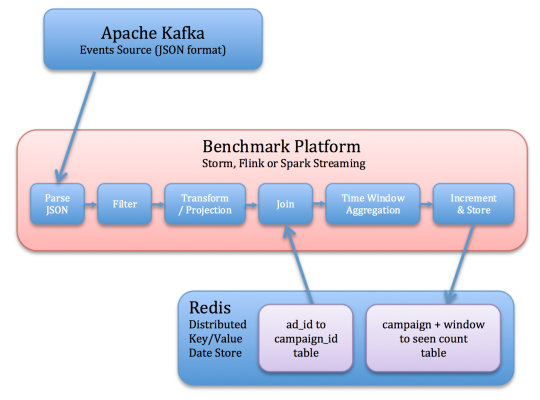
\includegraphics[scale=0.50]{images/yahoo_stream_bench}}
   \caption{Operations flow of YSB \cite{YSB}}
   \label{fig:yahoo_stream_bench}
  \end{center}
\end{figure}


The Yahoo Streaming Benchmark (YSB) is introduced to analysis what Storm is good at and where it needs to be improved compared to other stream processing systems by Yahoo storm team \cite{YSB}. The benchmark is a single advertisement application to identify relevant advertisement events. There are a number of advertising campaigns, and a number of advertisements for each campaign. The application need read various JSON events from a Kafka topic, identify the relevant events, and store a windowed count of relevant events per campaign into Redis. The flow of operations could be shown as Figure~\ref{fig:yahoo_stream_bench}.

Each event (message) in Kafka topic contains a timestamp marking the time producer created this event. Truncating this timestamp to a particular digit gives the begin-time of the time window that the event belongs in. When each window is updated in Redis, the last updated time is recored.

After each run, a utility reads windows from Redis and compares the windows' times to their last update times in Redis, yielding a latency data point. Because the last event for a window cannot have been emitted after the window closed but will be very shortly before, the difference between a window's time and its last update time minus its duration represents the time it took for the final tuple in a window to go from Kafka to Redis through the application. \\

$finalEventLatency = (lastUpdatedTime - createTime) - duration$

\begin{itemize}
  \item \textbf{finalEventLatency:} latency of an event; 
  \item \textbf{lastUpdatedTime:} the latest time that an event updated in Redis;
  \item \textbf{createTime:} the time when an event created; 
  \item \textbf{duration:} duration of a window.
\end{itemize}

More details about how the benchmark setup and the configuration of experiment environment could be found online~\footnote{\url{http://yahooeng.tumblr.com/post/135321837876/benchmarking-streaming-computation-engines-at}}. One shortcoming of this benchmark is one single workload could not reflect features of stream processing systems comprehensively, even the steps of benchmark flow attempt to probe common operations performed on data streams. Moreover, Redis is used to perform the join operator that could affect performance, therefore, there would be inaccuracy between the benchmark results and real performances of these stream processing systems. From experiments demonstrated in this page, Storm 0.10.0 was not able to handle throughputs above 135,000 events per second. The largest rate at which Kafka emitted data events into the Flink benchmark is varied 170,000 events/sec which doesn't reach throughput of Flink. The benchmark measures the latency of the frameworks under relatively low throughput scenarios, and establishes that both Flink and Storm can achieve sub-second latencies in these scenarios, while Spark Streaming has much higher latency.
%From the design and conclusion of experiments, it is very obvious that the benchmark focus more on latency other than throughput of stream processing systems.

To benchmark the real throughput of Flink, \citet{extend-YSB} reran YSB with some modifications that used the features in Flink to compute the windowed aggregates directly in Flink. In the last step of YSB, window updates to Redis is implemented with custom code with a separate user thread to flush results to Redis periodically on both Storm and Flink, which doesn't take advantage of Flink?s window API for computing windows. By reimplement the workload with Flink's window API, it came up with much better throughput numbers while still maintaining sub-second latencies. In StreamBench, we design a set of common APIs which are implemented with the best solution on different stream processing systems independently.
\clearpage




